\documentclass[a4,abstract=on]{scrartcl}

\usepackage[utf8]{inputenc}
\usepackage[T1]{fontenc}
\usepackage{placeins}
\usepackage{graphicx}
\usepackage[hypcap]{caption}
\usepackage{algorithm}
\usepackage[noend]{algpseudocode}
\usepackage[hidelinks]{hyperref}
\usepackage[nochapters]{classicthesis} % nochapters, wenn du section als oberste ebene nimmst
\usepackage{array}
\PassOptionsToPackage{big}{titlesec}

\floatname{algorithm}{Algorithmus}
% Mathe
\usepackage{amsmath}
\usepackage{amssymb}


% Verlinkungen
\usepackage[ngerman]{varioref} % Siehe http://en.wikibooks.org/wiki/LaTeX/Labels_and_Cross-referencing#The_varioref_package
%\usepackage[hidelinks]{hyperref}

% Spracheinstellungen sowie Umlaute etc.
\usepackage[ngerman]{babel}
\usepackage{ngerman}

% Bilder
\usepackage{graphicx}

% Tabellen-Abstand
\renewcommand{\arraystretch}{1.5}

% Quellcode
\usepackage{listings}
\lstset{%
	breaklines=true,
	frame=single,
	keepspaces=true,
	numbers=left,
	numbersep=5pt,
	tabsize=2
}

% Literatur
\usepackage{bibgerm}
\usepackage{natbib}

% Lässt sections immer auf der ungeraden (rechten) Seite anfangen.
    \newcommand*\stdsection{}
    \let\stdsection\section
    \renewcommand*\section{%
    \clearpage\ifodd\value{page}\else\mbox{}\clearpage\fi
    \stdsection}

% neuer Typ von Tabellenspalte (so wie c, l, etc.). Ist zentriert mit fester Breite.
\newcolumntype{C}[1]{>{\centering\let\newline\\\arraybackslash\hspace{0pt}}m{#1}}

% \usepackage{setspace}
% \onehalfspacing
\title{Untersuchung verschiedener Kodierungen von speziellen Cardinality Constraints für SAT}
\date{~}

\begin{document}
	\maketitle
\thispagestyle{empty}
\begin{center}
\begin{Large}
Bachelorarbeit\\Universität Bremen\\Fachbereich $3$\\
~\\~\\
\textbf{Jil Tietjen}\\<jiltietj@informatik.uni-bremen.de>\\
~\\~\\
Erstgutachter: Prof. Dr. Rolf Drechsler\\
Zweitgutachter: Prof. Dr. Rüdiger Ehlers\\~\\
\mbox{Betreuung: Prof. Dr. Rolf Drechsler \&~Oliver Keszöcze}\\~\\~\\~\\~\\~\\~\\~\\
Bremen, $09$. Juni $2016$
\end{Large}
\end{center}
		
	\newpage
~\\
\textbf{Urheberrechtliche Erklärung}\\
Erklärung gem. § $10$ ($10$) Allgemeiner Teil der BPO vom $27$.$10$.$2010$
Hiermit versichere ich, dass ich meine Bachelorarbeit ohne fremde Hilfe angefertigt habe, und dass ich keine anderen als die von mir angegebenen Quellen und Hilfsmittel benutzt habe.\\
Alle Stellen, die wörtlich oder sinngemäß aus Veröffentlichungen entnommen sind, habe ich unter Angabe der Quellen als solche kenntlich gemacht.\\
Die Bachelorarbeit darf nach Abgabe nicht mehr verändert werden.\\
~\\~\\~\\
Bremen, den $09$.$06$.$2016$\\
~\\~\\~\\
Jil Tietjen
~\\~\\~\\~\\~\\~\\
Ich bin damit einverstanden, dass meine Abschlussarbeit im Universitätsarchiv für wissenschaftliche Zwecke von Dritten eingesehen werden darf.\\
~\\~\\~\\
Bremen, den $09$.$06$.$2016$\\
~\\~\\~\\
Jil Tietjen
\clearpage

	\tableofcontents
	\clearpage

\section{Einleitung}
\section{Grundlagen}
\section{Kodierungen}
In diesem Kapitel werden die unterschiedlichen Kodierungen beschrieben. Das Ziel ist es, dass die Cardinality Constraints über die Menge der Boolschen Variablen in eine Konjunktive Normalform (KNF) gebracht werden. %Innerhalb der KNF gibt es Einschränkungen, die verlangen, dass höchstens $r$ der Booleschen Variablen 1 sein können. Rein in die Grundlagen
Das Cardinalitiy Constraint ist genau dann erfüllt, wenn die aus der Kodierung resultierende Formel erfüllt ist. Ein einzelnes Cardinality Constraint ist immer erfüllbar. Erst eine Kombination mehrerer Cardinality Constraints kann zu einer unerfüllbaren Formel führen.

%Evaluation Alle Kodierungen werden anhand des Damen-Problems und anhand einer Tomography auf ihre Praxistauglichkeit überprüft.

	\subsection{naiver Ansatz}
Zur Verdeutlichung der Einflüsse der weiteren Kodierungen wird als Erstes der naive Ansatz verfolgt. Bei dieser Methode wird aus allen möglichen Kombinationen die KNF gebildet. Das bedeutet, dass beispielsweise aus $x+y+z$ $(\neg x \vee \neg y) \wedge (\neg x \vee \neg z) \wedge (\neg z \vee \neg y)$ wird. Um alle Möglichkeiten auch bei einer grossen Anzahl von Variablen zu erfassen, wird als Grundlage die Mengenlehre angewendet. Es werden Untermengen erstellt, die sich mit folgendem System aufbauen. Das erste Element in der Menge bleibt immer gleich und für das zweite Element wird immer das nächst grössere Element ausgewählt. Eine Menge besteht immer aus den Teilmengen des ersten Index des Arrays vereinigt mit dem Element aus dem zweiten Index, aus dem dritten Index und so weiter. Dies wird rekursiv so lange fortgeführt bis alle Teilmengen erstellt sind. Die gebildete KNF kann schließlich mit $k$ verglichen werden.
%Todo Beweis für <= 1

	\subsection{Kodierung nach Bailleux und Boufkhad}
Im folgenden wird die Kodierung aus \cite[][]{bailleux} vorgetellt. Im weiteren Verlauf werden zusätzlich Formeln aus \cite[][]{knuth} hinzugezogen.
%Diese Kodierung ist, laut Bailleux, effizient mit Berücksichtigung der Unit Propagation, die in den meisten Sat-Solvern verwendet wird. Es werden O(n log (n)) Variablen und O($\text{n}^2$) Klauseln gefordert, die aus mindestens 3 Literalen bestehen. Bei dieser Kodierung ist das Besondere, dass es eine einstellige Darstellung von Integer-Variablen gibt, die nicht nur den Wert an sich repräsentieren, sondern auch einem Intervall zugeordnet werden kann. Zum Beispiel gilt die Variable c nur, wenn das Intervall der Variablen ($a + b$) c erfüllt. Dadurch erhält man eine KNF. Die Kodierung muss korrekt sein, wenn es eine wahre Zuordnung gibt die unter der Berücksichtigung der Constraints erfüllbar ist.

%n erklären in den Grundlagen
Bei dieser Kodierung soll ein binärer Baum aufgebaut werden. Aus dem binären Baum können anhand von Formeln Literale gebildet werden. Durch das Wegstreichen von trivialen Variablen bleiben am Ende einige Klauseln mit einem Literal übrig. Für diese Literale kann sehr schnell eine Belegung gefunden werden. Dies steigert die Effizienz der Kodierung.

Der Baum wird iterativ aufgebaut und beginnt mit einem Wurzelknoten, der mit $1$ betitelt wird. Des Weiteren gibt es $n-1$ interne Knoten, sowie $n$ Blätter, die von $n$ bis $2n-1$ beschriftet werden. Die Kinder von Knoten $k$  für $1 \leq k \textless n$, sind die Knoten $2k$ und $2k +1$. Dies wird so lange wiederholt bis das letzte Blatt erreicht ist.
Jedem Knoten wird eine Menge von Variablen zugeordnet. Dabei wird jedem Blatt eine Eingangsvariable und dem Wurzelknoten eine Menge von Ausgangsvariablen zugeordnet. Nun wurd die Kodierung so aufgebaut, dass die Variablen eines inneren Knotens die Summe der Variablen seiner Kindsknoten repräsentieren. Daraus ergibt sich ein Wurzelknoten dessen Variablen mit $r$ verglichen werden können, da sie die Summe aller Eingangsvariablen repräsentieren.\\

Als nächster Schritt werden neue Variablen der Form $\text{b}_j^k$ gebildet, für $1 \textless k \textless n$ und  $1 \leq j \leq t_k$ werden Hilfesvariablen $ b_j^k$ erzeugt. Das Minimum von r und die Anzahl der Blätter unter dem Knoten k ist dabei $t_k$. Bei $n=2$ hat der Knoten $1$ zum Beispiel $2$ Blätter, daher ist $t_1=2$. Jedem inneren Knoten k wird die Menge der Variablen $\text{b}_j^k$ zugeordnet.\\
Mit den neuen Variablen können folgende Klauseln gebildet werden:\\
\textbf{1. Formel:}\\
$ \neg \text{b}_i^{2k} \vee \neg \text{b}_j^{2k+1} \vee \neg \text{b}_{i+j}^{k}$ \\
für $0\leq i \leq \text{t}_{2k}$, $0\leq j \leq \text{t}_{2k+1}$, $1\leq i+j \leq \text{t}_{k}+1$, $1\textless k \textless n$\\
\textbf{2. Formel:}\\
$ \neg \text{b}_i^2 \vee \neg \text{b}_j^3$ für $0\leq i \leq \text{t}_2$, $0\leq j \leq \text{t}_3$, $i+j = r+1$\\

Dabei wird $\text{t}_k$ zu $1$ und $\text{b}_1^k = \text{x}_{k-n+1}$ für $n \leq k \textless 2n$. Dadurch können aus den Hilfsvariablen die entsprechenden Literale gebildet werden, die die KNF bilden.
Aufgrund des Aufbaus der Formel können Variablen der Form $\text{b}_(r+1)^k$ nur positiv und Variablen der Form $\text{b}_0^k$ nur negativ vorkommen. Daher können diese Variablen gestrichen werden.

\subsubsection{Beispiel für die Kodierung}
Für das Beispiel ist $n=4$ und $r =1$. Der binäre Baum hat $4-1 = 3$ interne Knoten, sowie 4 Blätter, die beschriftet sind mit 4 bis $2*4-1=7$. Die Kinder von Knoten $1$  für $1 \leq 1 \textless 4$, sind die Knoten 2 und $2*1 +1=3$. Daraus ergibt sich der binäre Baum, der in Abbildung \ref{fig:baum} zu sehen ist.

\begin{figure}[H]
\centering
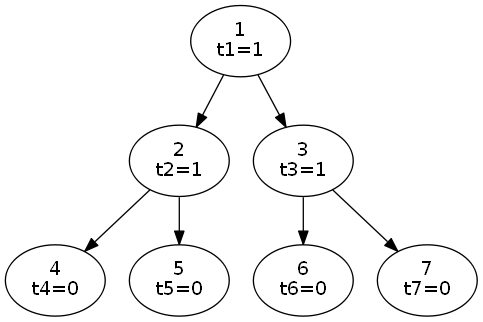
\includegraphics[width=9cm]{bailleux.png}
\caption{Binärer Baum nach Bailleux}
\label{fig:baum}
\end{figure}

Der Knoten $1$ hat die Blätter $4,5,6$ und $7$. Daher müsste $\text{t}_1 = 4$ sein, da es aber das Minimum von $r$ sein soll, ist $t_1=1$. Die weiteren Variablen $\text{t}_2$ und $\text{t}_3$ sind auch jeweils $1$ und $\text{t}_4$ bis $\text{t}_7$ hat keine Blätter und sind somit $0$.

Dadurch ergeben sich für das Beispiel von $n=4$ folgende Variablen:\\
\textbf{Formel 1:}\\
$k=2$ oder $k=3$, weil $1 \textless k \textless n$.\\
$j=0$ oder $j=1$, weil $1 \leq j \leq \text{t}_k$ und $\text{t}_k = 1$.\\
$i=0$ oder $i=1$, weil $1\leq i+j \leq \text{t}_{k}+1$.\\
Somit ergeben sich für (i,j) die Möglichkeiten $(1,0)$, $(0,1)$ und $(1,1)$.\\
\textbf{k = 2:}\\
$\neg \text{b}_1^4 \vee \neg \text{b}_0^5 \vee \text{b}_1^2$\\
$\neg \text{b}_0^4 \vee \neg \text{b}_1^5 \vee \text{b}_1^2$\\
$\neg \text{b}_1^4 \vee \neg \text{b}_1^5 \vee \text{b}_2^2$\\
\textbf{k = 3:}\\
$\neg \text{b}_1^6 \vee \neg \text{b}_0^7 \vee \text{b}_1^3$\\
$\neg \text{b}_0^6 \vee \neg \text{b}_1^7 \vee \text{b}_1^3$\\
$\neg \text{b}_1^6 \vee \neg \text{b}_1^7 \vee \text{b}_2^3$\\

Da alle der Form $\neg \text{b}_0^k$ und $\text{b}_{r+1}^k$  gestrichen werden, bleiben nur noch diese Variablen übrig:\\
\textbf{k = 2:}\\
$\neg \text{b}_1^4  \vee \text{b}_1^2$\\
$\neg \text{b}_1^5 \vee \text{b}_1^2$\\
$\neg \text{b}_1^4 \vee \neg \text{b}_1^5$\\
\textbf{k = 3:}\\
$\neg \text{b}_1^6 \vee \text{b}_1^3$\\
$\neg \text{b}_1^7 \vee \text{b}_1^3$\\
$\neg \text{b}_1^6 \vee \neg \text{b}_1^7 $\\

Folgende Literale können gebildet werden:\\
$\neg \text{b}_1^4 = \neg \text{x}_1$, weil $\text{x}_{4-4+1}=\text{x}_1$ ist.\\
 Alle anderen Variablen werden zu:\\
$ \neg \text{x}_1 \vee \text{b}_1^2$\\
$\neg \text{x}_2 \vee  \text{b}_1^2$\\
$\neg \text{x}_1 \vee \neg \text{x}_2$\\
$\neg \text{x}_3 \vee \text{b}_1^3$\\
$\neg \text{x}_4 \vee \text{b}_1^3$\\
$\neg \text{x}_3 \vee \neg \text{x}_4$\\

\textbf{Formel 2:}\\
$i=1$, weil $0\leq i \leq \text{t}_2$ für $\text{t}_2 = 1$.\\
$j=1$, weil $0\leq j \leq \text{t}_3$ für $\text{t}_3=1$.\\
Somit ergeben sich für (i,j) die Möglichkeiten $(1,1)$, so dass $i+j = r+1$ gilt.\\
$\neg \text{b}_1^2 \vee \neg \text{b}_1^3$\\

Es können keine Variablen gestrichen werden.\\

Die vollständige KNF sieht folgendermaßen aus:\\
($ \neg \text{x}_1 \vee \text{b}_1^2$) $\wedge$ ($\neg \text{x}_2 \vee \text{b}_1^2$) $\wedge$ ($\neg \text{x}_1 \vee \neg \text{x}_2$) $\wedge$ ($\neg \text{x}_3 \vee \text{b}_1^3$) $\wedge$ ($\neg \text{x}_4 \vee \text{b}_1^3$) $\wedge$ ($\neg \text{x}_3 \vee \neg \text{x}_4$) $\wedge$ ($\neg \text{b}_1^2 \vee \neg \text{b}_1^3$)\\

	\subsection{Kodierungen nach Sinz}
Dieses Kapitel behandelt zwei Kodierungen nach Sinz, die auf einen sequentiellen Counter und einem parallelen Counter basieren \cite[][]{sinz}. Grundlegend besteht diese Kodierung aus einem Schaltkreis, der die Summe die Eingangsvariablen mit Hilfe eines ein- oder zweistelligen Counters bildet und das Ergebnis mit $r$ vergleicht. Die Unterschiede der Schaltkreise werden im weiteren Verlauf beschrieben.
		\subsubsection{sequentiell}
Die sequentlielle Variante besteht aus zwei aufeinander folgende Stufen. In der ersten Stufe werden die Inputs gezählt, die auf true gesetzt werden. In der nächsten Stufe überprüft ein Comparator, ob das Zählerergebnis innerhalb von $r$ liegt (siehe Abbildung \ref{fig:sinz_counter}). Der Counter besteht aus mehreren Sub-Schaltkreisen und in jedem Sub-Schaltkreis wird die nächste Eingangsvariable addiert. Daher kann die komplette Summe erst im letzten Sub-Schaltkreis berechnet werden. \\


\begin{figure}[H]
\centering
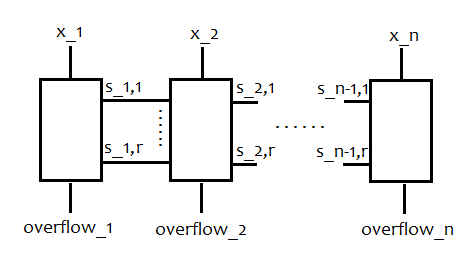
\includegraphics[width=\textwidth]{Sinz_seq.png}
\caption{Sequentieller Counter von Sinz in Anlehnung an \cite[][] {sinz}}
\label{fig:sinz_counter}
\end{figure}

Jeder Addierer erhält eine Eingangsvariable und $r$-viele Teilsummen als Eingänge. Es gibt $n$ Addierer und bei jedem geht ein Overflow-Bit heraus. Die entstehenden Überträge der einzelnen Addierer werden auf true gesetzt, wenn die Teilsumme größer als $r$ ist. Damit die Cardinality Constraints erfüllbar sein können, sind keine Überträge erlaubt, somit werden sie auf false gesetzt. Diese Aufgabe übernimmt schon der Comparator. Es wird ausgenutzt, dass $\neg \text{overflow}_i$ für $1 \leq i \leq n$ gelten muss, um den Schaltkreis zu vereinfachen. Daraus ergeben sich dann eine Menge von Klauseln.

Bei dieser Variante werden erneut anhand von \cite[][]{knuth} neue Variablen eingeführt. Dafür müssen $n$ und $r$ wieder bekannt sein, wie bei Bailleux und Boufkhad. Es werden $(n-r)*r$ neue Variablen der Form $\text{s}_j^k$ für $1 \leq j \leq n - r$ und $1 \leq k \leq r$ gebildet. \\
Mit den neuen Variablen können folgende Klauseln erstellt werden:\\
\textbf{1. Formel:}\\
$(\neg \text{s}_j^k \vee \text{s}_{j+1}^k)$ für $(1 \leq j \textless n - r)$ und $(1 \leq k \leq r)$\\
\textbf{2. Formel:}\\
$(\neg \text{x}_{j+k} \vee \neg \text{s}_j^k \vee \text{s}_j^{k+1})$ für $1 \leq j \leq n - r$ und $0 \leq k \leq r$\\

Die Variablen der Form  $\neg s_j^0$ können gestrichen werden. Es bedetuet, dass die Teilsumme vom $j-ten$ Sub-Schaltkreis  $0$ ist. $0$ hätte keine Auswirkung auf den Vergleich mit $r$ und ist daher überflüssig. Des Weiteren dürfen Variablen der Form $\text{s}_j^{r+1}$ gestrichen werden, weil dies auf jeden Fall größer als $r$ wäre und somit niemals eine Belegung für gefunden werden könnte.

	\subsubsection{Beispiel für eine sequentielle Kodierung}
Es ergeben sich für das Beispiel von $n=4$ und $r=1$ folgende Variablen:\\
\textbf{Formel 1:}\\
Da $1 \leq j \textless 3$ ergeben sich $1$ oder $2$ für j.\\
Für $k$ ergibt sich $1$, da $1 \leq k \leq 1$.\\
$\neg \text{b}_1^1 \vee \text{b}_2^1$\\
$\neg  \text{b}_2^1 \vee \text{b}_3^1$\\
In diesem Fall können keine Variablen gestrichen werden.\\

\textbf{Formel 2:}\\
Bei dieser Formel kann j $1, 2$ oder $3$ sein, da $1 \leq j \leq 3$ . Die Variable $k$ kann $0$ oder $1$ sein, da $0 \leq k \leq 1$.\\
\textbf{k = 0:}\\
$\neg x_1 \vee \neg b_1^0 \vee b_1^1$\\
$\neg x_2 \vee \neg b_2^0 \vee b_2^1$\\
$\neg x_3 \vee \neg b_3^0 \vee b_3^1$\\
\textbf{k =1:}\\
$\neg x_2 \vee \neg b_1^1 \vee b_1^2$\\
$\neg x_3 \vee \neg b_2^1 \vee b_2^2$\\
$\neg x_4 \vee \neg b_3^1 \vee b_3^2$\\

Alle trivialen Variablen werden gestrichen. Diese Klauseln bleiben bestehen:\\
\textbf{k = 0:}\\
$\neg x_1 \vee b_1^1$\\
$\neg x_2 \vee b_2^1$\\
$\neg x_3 \vee b_3^1$\\
\textbf{k =1:}\\
$\neg x_2 \vee \neg b_1^1 $\\
$\neg x_3 \vee \neg b_2^1 $\\
$\neg x_4 \vee \neg b_3^1 $\\

Die vollständige KNF sieht folgendermaßen aus:\\
$(\neg b_1^1 \vee b_2^1) \wedge (\neg b_2^1 \vee b_3^1) \wedge (\neg x_1 \vee b_1^1) \wedge (\neg x_2 \vee b_2^1) \wedge (\neg x_3 \vee b_3^1) \wedge (\neg x_2 \vee \neg b_1^1) \wedge (\neg x_3 \vee \neg b_2^1) \wedge (\neg x_4 \vee \neg b_3^1) $\\

		\subsubsection{parallel}
Der Unterschied zum sequentiellen Counter besteht darin, dass beim parallelen Counter die Eingangsvariablen in zwei Hälften geteilt werden und durch Sub-Counter parallel verarbeitet werden können. Die erste Hälfte bildet sich durch $2^m$ und muss grösser sein als die zweite Hälfte. Daher wird die zweite Hälfte durch $2^{m+1}$ berechnet. In beiden Fällen bildet sich $m$ durch den Logarithmus von n und $m$ muss so gewäht werden, dass folgende Bedingung erfüllt ist $2^m \leq n \textless 2^{m+1}$. Damit die zweite Hälfte nie weniger Eingangsvariablen enthält als die erste, gibt es den Sonderfall, dass die zweite Hälfte keine Eingangsvariablen hat. Gibt es nur eine oder zwei Eingangsvariablen, gehen die Inputs sofort in den Halbaddierer als CarryIn und Eingangsvariable.\\
Im nächsten Schritt wird rekursiv in den Countern berechnet wie gross die Anzahl der Eingangsvariablen ist, die auf true gesetzt werden müssen. Dabei sind die Counter der ersten Hälfte Halbaddierer und die Counter der zweiten Hälfte 1-Bit-Volladdierer. Die letzte Einganzsvariable wird als Carry-Bit in den Counter gegeben. Die parallelen Counter berechnen somit die Summe von $2^m-1$ Eingangsvariablen.\\

\begin{figure}[H]
\centering
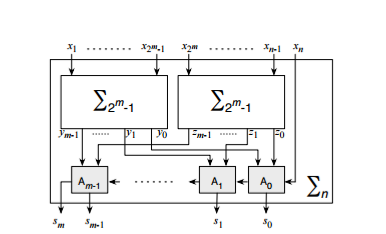
\includegraphics[width=9cm]{Sinz_para.png}
\caption{Paralleler Counter von Sinz (siehe \cite[][] {sinz}, Seite 9)}
\label{fig:sinz_counter_para}
\end{figure}

Bei den Volladdierern wird ausgenutzt, dass jeder Output einen weniger hat als es Inputs gab. Somit können Leitungen reduziert werden. Des Weiteren kann durch die Anzahl der Eingangsvariablen ($n$) und den $m+1$ Outputs gesagt werden, dass der Schaltkreis aus $n-(m+1)$ Volladdierern besteht. Die Anzahl der Halbaddierer kann ebenfalls berechnet werden, indem die Nullen in der binären Repräsentation der Eingangsvariablen ($n$) gezhählt werden. Die Anzahl müsste kleiner oder gleich $m$ sein.\\

Der Halb-Addierer und Voll-Addierer kann folgendermaßen als KNF ausgedrückt werden:\\
Der Halb-Addierer besteht aus drei Klauseln:
\begin{itemize}
\item $(a \vee \neg carryIn \vee sum)$
\item $(\neg a \vee carryIn \vee sum)$
\item $(\neg a \vee \neg caaryIn \vee carryOut )$
\end{itemize}

Der Voll-Addierer besteht aus sieben Klauseln:
\begin{itemize}
\item $(a \vee b \vee \neg carryIn \vee sum)$
\item $( a \vee \neg b \vee carryIn \vee sum)$
\item $(\neg a \vee b \vee caaryIn \vee sum )$
\item $(\neg a \vee \neg b \vee \neg carryIn \vee sum)$
\item$(\neg a \vee \neg b \vee carryOut)$
\item$(\neg a \vee \neg carryIn \vee carryOut)$
\item$(\neg b \vee carryIn \vee carryOut)$
\end{itemize}

Zum Schluss wird noch ein Comparator benötigt, damit die Cardinality Constraints mit $k$ vergllichen werden können. Dieser stellt sicher, dass das Ergebnis nicht grösser ist als $k$. Dafür wird $k$ als binäre Repräsentation dargestellt, so dass die Belegung der Outputs mit der binären Repräsentation von $k$ verglichen werden kann.

\subsubsection{Beispiel für eine parallele Kodierung}
Für dieses Beispiel wird $n=9$ gesetzt, so dass $2^3 \leq 9 \textless 2^4$ ist. Somit ergibt sich für dieses Beispiel, dass es Volladdierer und Halbaddierer gibt. Der Aufbau der Schaltkreise wird in den folgenden Bildern dargestellt.

\begin{figure}[H]
\centering
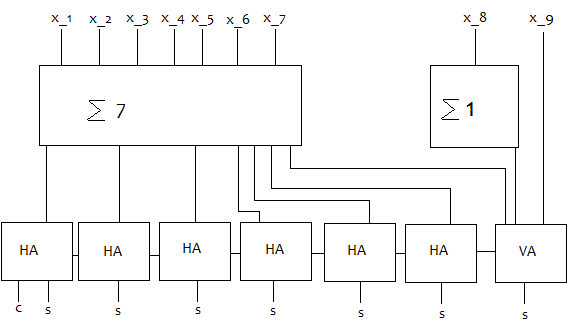
\includegraphics[width=\textwidth]{Bsp_Sinz_grob.png}
\caption{Paralleler Counter von Sinz für $n=9$}
\label{fig:sinz_counter_para_bsp}
\end{figure}

Durch die hohe Summe für die erste Hälfte der Eingangsvariablen ($\sum7$) wird der Schaltkreis weiter unterteilt dargestellt.

\begin{figure}[H]
\centering
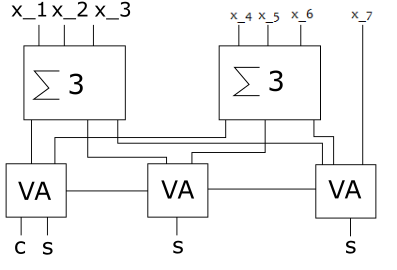
\includegraphics[width=\textwidth]{Bsp_Sinz_fein.png}
\caption{Paralleler Counter von Sinz}
\label{fig:sinz_counter_para_bsp}
\end{figure}

Das Beispiel besteht aus 11 Volladdierern sowie 6 Halbaddierern und aus 95 Klauseln für den Schaltkreis.\\

\textbf{Beispiel für den Comparator anhand von $k$}:\\
$k = 18$, in binärer Repräsenation ist dies $10010$. Daraus ergeben sich 3 Klauseln, da es drei Nullen gibt und 5 verschiedene Variablen, bei denen die Variablen mit einer $0$ nur negiert aufgeschrieben werden. Das bedeutet, dass $1=x_4, 0=x_3, 0=x_2, 1=x_1$ und $0=x_0$.\\
Die folgenden Klauseln können gebildet werden:\\
\begin{itemize}
\item $\{\neg x_0\}$ (Variale wird nur negiert aufgeschrieben)
\item  $\{\neg x_0,\neg x_1\}$ (Variable wird in alle bestehenden Mengen hinzugefügt)
\item $\{\{\neg x_0, \neg x_1\},\{\neg x_2\}\}$
\item $\{\{\neg x_0, \neg x_1\},\{\neg x_2\}, \{\neg x_3\}\}$
\item $\{\{\neg x_0, \neg x_1\, \neg x_4\},\{\neg x_2, \neg x_4\}, \{\neg x_3, \neg x_4\}\}$
\end{itemize}


	\subsection{naive Kodierung basierend auf Sorting Networks}
	\subsection{Sorting Networks mit odd-even Mergesort}
	\subsection{Kodierung basierend auf BDDs}

	\subsection{Entwickelte Kodierung mit Sorting Networks}

\section{Umsetzung}
 Als Testproblem für die unterschiedlichen Kodierungen wird das n-Damen-Problem verwendet, da dieses Problem eine wichtige Rolle in der Informatik spielt und viele Constraints abgeleitet werden können. In jeder Reihe (vertikal, horizontal und diagonal) ist nur eine Dame erlaubt. Somit ergeben sich unterschiedliche Kombinationen, die für die Belegung der Literale nur erlaubt sind. Ziel ist es eine Belegung zu finden, die alle Bedingungen erfüllt. 

\begin{figure}[H]
\centering
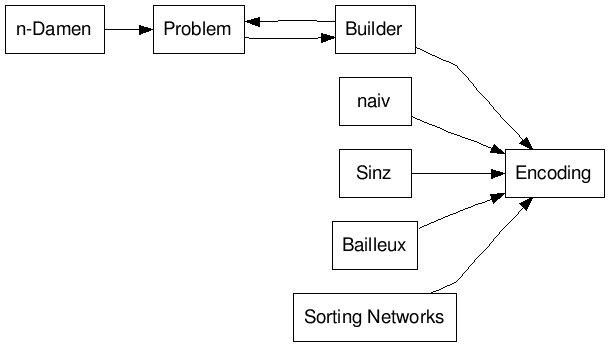
\includegraphics[width=\textwidth]{architektur.png}
\caption{Die Architektur der Implementierung}
\label{fig:architektur}
\end{figure}

In Abbildung \ref{fig:architektur} ist dargestellt, wie die grundlegende Architektur aufgebaut ist. 
Der Builder ist die Zwischenschicht zwischen den Problemen und den unterschiedlichen Kodierungen. Er erstellt das Encoding und ermöglicht dadurch den Aufruf verschiedener Kodierungen. In dieser Klasse werden die verschiedenen Constraints für $\leq$, 	$\geq$ und $\doteq$ gebaut und der Solver wird aufgerufen. Die Klasse Encoding dient als Oberklasse und ist abstrakt, damit die Signatur für die Unterklassen (Kodierungen) vorgegeben ist. 

\section{Evaluation}

\section{Schlussfolgerung und Ausblick}

%Sogar zitieren kann man \textbackslash o/ \cite[vgl.][]{invincible}.


%\begin{algorithm}
%\caption{Minimax-Suche}
%\label{alg:minimax}
%\begin{algorithmic}
%\State $\text{minimax(Spielstellung s)}$
%\State $\text{~~~~falls }spielende(s)$
%\State $\text{~~~~~~~~return }payoff(s)$
%\State $\text{~~~~} v \gets -\infty$
%\State $\text{~~~~für alle möglichen Züge }m$
%\State $\text{~~~~~~~~} f"uhreZugAus(s, m)$
%\State $\text{~~~~~~~~} v' \gets -minimax(s)$
%\State $\text{~~~~~~~~} nimmZugZur"uck(s, m)$
%\State $\text{~~~~~~~~falls }v' > v$
%\State $\text{~~~~~~~~~~~~}v \gets v'$
%\State $\text{~~~~return } v$
%\end{algorithmic}
%\end{algorithm}

%\begin{table}
%\centering
%\small %macht die Schrift kleiner
%\setlength{\tabcolsep}{.11cm} %macht den seitlichen Rand der Zellen kleiner (und damit die Tabelle schmaler)
%\begin{tabular}{|c||c|c|c|C{1.3cm}|c||c|}
%\hline
% & Base & Setup & Heuristics & Chance Pruning & Extensions & Gesamt \\ \hline \hline
%Base & - & $20$ & $22$ & $16,5$ & $18,5$ & $77$\\ \hline
%Setup & $30$ & - & $23,5$ & $19,5$ & $23$ & $96$\\ \hline
%Heuristics & $28$ & $26,5$ & - & $19,5$ & $23,5$ & $97,5$ \\ \hline
%ChancePruning & $33,5$ & $30,5$ & $30,5$ & - & $27$ & $121,5$\\ \hline
%Extensions & $31,5$ & $27$ & $26,5$ & $23$ & - & $108$ \\ \hline
%\end{tabular}
%\caption{Paarweise Ergebnisse des Turniers}
%\label{tab:roundrobin}
%\end{table}

	\clearpage
	\appendix
	\section{Literaturverzeichnis}
		% Latex-Magie von http://tex.stackexchange.com/questions/22645/hiding-the-title-of-the-bibliography
		\begingroup
			\renewcommand{\section}[2]{}
			\bibliographystyle{natdin}
			\bibliography{referenzen}
		\endgroup
\clearpage
	\section{Abbildungsverzeichnis}
		\begingroup
			\renewcommand{\section}[2]{}
			\listoffigures
		\endgroup
	\section{Tabellenverzeichnis}
		\begingroup
			\renewcommand{\section}[2]{}
			\listoftables
		\endgroup
\end{document}
